% Figure 6 composite (vector). Build: lualatex fig6_assemble.tex
%
% Layout rules applied (Nature Methods, 2026-07-27 rework):
%   * page 183 mm wide, 159.0 mm tall (was 187 mm: panel g no longer needs half
%     the page, because it now starts at the decision node instead of redrawing
%     panel a's three pilot steps).
%   * every panel in a row is scaled to ONE common row height, so each row shares
%     a common top edge and a common baseline; horizontal gutters are exactly
%     5.0 mm in both rows and the vertical gutters are exactly 6.0 mm.
%     row 1 height 44.306 mm, row 2 height 42.642 mm.
%   * content block runs 4.5 mm to 180.5 mm; panel letters sit 3.2 mm to the left
%     of each panel's left edge, on the panel's top edge.
%   * panel letters: lowercase bold 8 pt at final size (the previous
%     \bfseries\large rendered at ~12 pt).
%   * panel g is drawn in matplotlib at 168 x 52 mm and placed at 176 mm
%     (scale 1.048), so its in-panel type is 5.7 pt or larger on the page.
\documentclass[tikz,border=1mm]{standalone}
\usepackage{graphicx}
% Shared font contract for every AllelePerturb composite (Nature Methods).
% Input from each figN_assemble.tex as % Shared font contract for every AllelePerturb composite (Nature Methods).
% Input from each figN_assemble.tex as % Shared font contract for every AllelePerturb composite (Nature Methods).
% Input from each figN_assemble.tex as \input{../nm_fonts.tex}.
%
% ONE sans family per figure. The matplotlib panels resolve their family through
% nm_style.py as Arial -> Helvetica -> Liberation Sans (first installed wins), so
% the panel letters stamped by figN_assemble.tex must resolve the same way or the
% composite embeds two families. Until 2026-07-31 these files loaded helvet, which
% put NimbusSanL (a Helvetica clone, Type 1) in every composite for the letters
% while every other glyph was Liberation Sans (an Arial clone, CID TrueType).
% Nature Methods asks for Arial or Helvetica; it does not accept both in one figure.
%
% Requires lualatex, i.e. fontspec + luaotfload (Debian/Ubuntu: texlive-luatex).
% Build every composite with:
%     lualatex -interaction=nonstopmode figN_assemble.tex
% pdflatex will fail here by design: it cannot load a system OpenType/TrueType
% family, and silently falling back to helvet is the defect this file removes.
\usepackage{fontspec}
\IfFontExistsTF{Arial}%
  {\setsansfont{Arial}}%
  {\IfFontExistsTF{Helvetica}%
     {\setsansfont{Helvetica}}%
     {\setsansfont{Liberation Sans}}}
\renewcommand{\familydefault}{\sfdefault}
.
%
% ONE sans family per figure. The matplotlib panels resolve their family through
% nm_style.py as Arial -> Helvetica -> Liberation Sans (first installed wins), so
% the panel letters stamped by figN_assemble.tex must resolve the same way or the
% composite embeds two families. Until 2026-07-31 these files loaded helvet, which
% put NimbusSanL (a Helvetica clone, Type 1) in every composite for the letters
% while every other glyph was Liberation Sans (an Arial clone, CID TrueType).
% Nature Methods asks for Arial or Helvetica; it does not accept both in one figure.
%
% Requires lualatex, i.e. fontspec + luaotfload (Debian/Ubuntu: texlive-luatex).
% Build every composite with:
%     lualatex -interaction=nonstopmode figN_assemble.tex
% pdflatex will fail here by design: it cannot load a system OpenType/TrueType
% family, and silently falling back to helvet is the defect this file removes.
\usepackage{fontspec}
\IfFontExistsTF{Arial}%
  {\setsansfont{Arial}}%
  {\IfFontExistsTF{Helvetica}%
     {\setsansfont{Helvetica}}%
     {\setsansfont{Liberation Sans}}}
\renewcommand{\familydefault}{\sfdefault}
.
%
% ONE sans family per figure. The matplotlib panels resolve their family through
% nm_style.py as Arial -> Helvetica -> Liberation Sans (first installed wins), so
% the panel letters stamped by figN_assemble.tex must resolve the same way or the
% composite embeds two families. Until 2026-07-31 these files loaded helvet, which
% put NimbusSanL (a Helvetica clone, Type 1) in every composite for the letters
% while every other glyph was Liberation Sans (an Arial clone, CID TrueType).
% Nature Methods asks for Arial or Helvetica; it does not accept both in one figure.
%
% Requires lualatex, i.e. fontspec + luaotfload (Debian/Ubuntu: texlive-luatex).
% Build every composite with:
%     lualatex -interaction=nonstopmode figN_assemble.tex
% pdflatex will fail here by design: it cannot load a system OpenType/TrueType
% family, and silently falling back to helvet is the defect this file removes.
\usepackage{fontspec}
\IfFontExistsTF{Arial}%
  {\setsansfont{Arial}}%
  {\IfFontExistsTF{Helvetica}%
     {\setsansfont{Helvetica}}%
     {\setsansfont{Liberation Sans}}}
\renewcommand{\familydefault}{\sfdefault}

\begin{document}
\begin{tikzpicture}[x=1mm,y=1mm]
  \useasboundingbox (0,0) rectangle (183,159.0);
  % ---- row 1 (common height 44.306 mm): a triage schematic | b LODO ROC | c AUROC forest
  \node[anchor=north west,inner sep=0] at (4.50,156.00)  {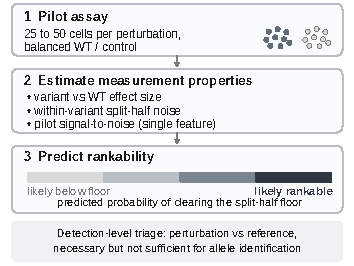
\includegraphics[width=59.07mm]{fig6a_pipeline.pdf}};
  \node[anchor=north west,inner sep=0] at (68.57,156.00) {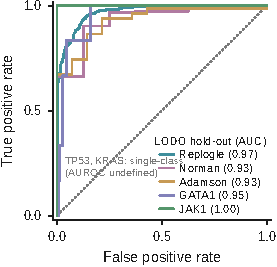
\includegraphics[width=45.94mm]{fig6b_roc.pdf}};
  \node[anchor=north west,inner sep=0] at (119.51,156.00){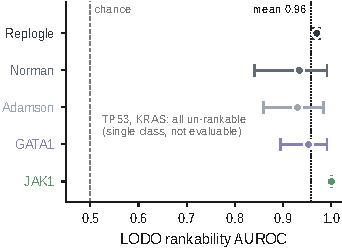
\includegraphics[width=60.99mm]{fig6c_auroc.pdf}};
  % ---- row 2 (common height 42.642 mm): d prospective | e design landscape | f depth-match
  \node[anchor=north west,inner sep=0] at (4.50,105.69)  {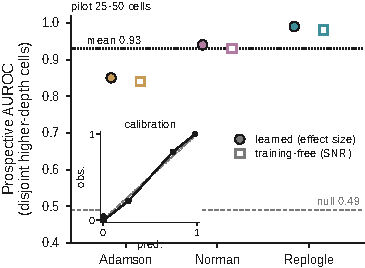
\includegraphics[width=58.09mm]{fig6d_prospective.pdf}};
  \node[anchor=north west,inner sep=0] at (67.59,105.69) {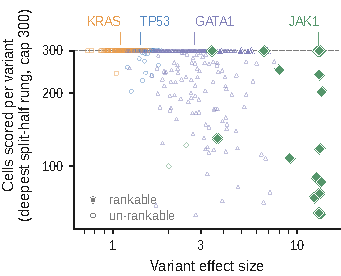
\includegraphics[width=52.73mm]{fig6e_design.pdf}};
  \node[anchor=north west,inner sep=0] at (125.33,105.69){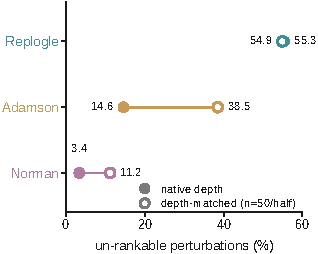
\includegraphics[width=55.17mm]{fig6f_depthmatch.pdf}};
  % ---- row 3: g power-aware reporting protocol (decision half), full content width
  \node[anchor=north west,inner sep=0] at (4.50,57.05)   {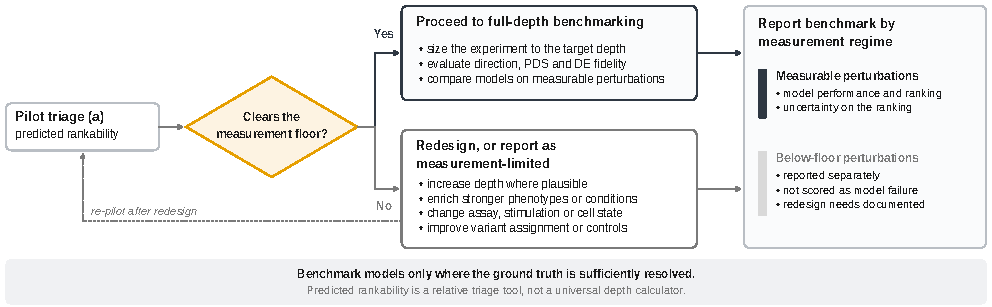
\includegraphics[width=176mm]{fig6g_workflow.pdf}};
  % ---- panel letters: lowercase, bold, 8 pt at final size
  \tikzset{plab/.style={font=\fontsize{8}{9}\selectfont\bfseries,anchor=north west,inner sep=0}}
  \node[plab] at (1.30,157.00) {a};  \node[plab] at (65.37,157.00) {b};  \node[plab] at (116.31,157.00) {c};
  \node[plab] at (1.30,106.69) {d};  \node[plab] at (64.39,106.69) {e};  \node[plab] at (122.13,106.69) {f};
  \node[plab] at (1.30,58.05)  {g};
\end{tikzpicture}
\end{document}
